\section{Exercises}

\begin{exercise}
    \label{exercise:linear_sharp_inequality}
    In the simple case where $\mat A$ is symmetric,
    find values of $\vect x$, $\vect b$ and $\Delta \vect b$ for which the inequality~\eqref{eq:linear_perturbation_rhs} is in fact an equality?
\end{exercise}

\begin{exercise}
    [Inverse of Gaussian transformation]
    \label{exercise:inverse_gaussian_transformation}
    Prove the formula~\eqref{eq:inverse_gaussian_transformation}.
\end{exercise}

\begin{exercise}
    \label{exercise:linear_product_of_lower_triangular}
    Prove that the product of two lower triangular matrices is lower triangular.
\end{exercise}

\begin{exercise}
    \label{exercise:linear_positive_definite_matrix_nonsingular_principal_components}
    Assume that $\mat A \in \real^{n \times n}$ is positive definite,
    i.e.\ that
    \[
        \forall \vect x \in \real^n \backslash \{ \vect 0_n \}, \qquad \vect x^\t \mat A \vect x > 0.
    \]
    Show that all the principal submatrices of $\mat A$ are nonsingular.
\end{exercise}

\begin{compexercise}
    Implement the backward substitution algorithm for solving $\mat U x = y$.
    What is the computational cost of the algorithm?
\end{compexercise}

\begin{compexercise}
    \label{exercise:linear_lu_with_partial_pivoting}
    Compare the condition number of the matrices $\mat L$ and $\mat U$ with and without partial pivoting.
    For testing, use a matrix with pseudo-random entries generated as follows
    \begin{minted}{julia}
    import Random
    # Set the seed so that the code is deterministic
    Random.seed!(0)
    n = 1000 # You can change this parameter
    A = randn(n, n)
    \end{minted}
\end{compexercise}
\begin{solution}
    See the Jupyter notebook for this chapter.
\end{solution}

\begin{compexercise}
    \label{exercise:linear_cholesky}
    Write a code for calculating the Cholesky factorization of a symmetric positive definite matrix $\mat A$ by comparing the entries of the product $\mat C \mat C^\t$ with those of the matrix $\mat A$.
    What is the associated computational cost,
    and how does it compare with that of the $\mat L \mat U$ factorization?

    \noindent \textbf{Extra credit:} ... if your code is able to exploit the potential banded structure of the matrix passed as argument for better efficiency.
    Specifically, your code will be tested with a matrix is of the type \julia{BandedMatrix} defined in the \texttt{BandedMatrices.jl} package,
    which you will need to install.
    The following code can be useful for testing purposes.
    \begin{minted}{julia}
    import BandedMatrices
    import LinearAlgebra

    function cholesky(A)
        m, n = size(A)
        m != n && error("Matrix must be square")
        # Convert to banded matrix
        B = BandedMatrices.BandedMatrix(A)
        B.u != B.l && error("Matrix must be symmetric")
        # --> Your code comes here <--
    end
    n, u, l = 20000, 2, 2
    A = BandedMatrices.brand(n, u, l)
    A = A*A'
    # so that A is symmetric and positive definite (with probability 1).
    C = @time cholesky(A)
    LinearAlgebra.norm(C*C' - A, Inf)
    \end{minted}
    For information, my code takes about 1 second to run with the parameters given here.
\end{compexercise}

\begin{exercise}
    [Matrix square root]
    \label{exercise:matrix_square_root}
    Let $\mat A \in \real^{n\times n}$ be a symmetric positive definite matrix.
    Show that $\mat A$ has a positive definite square root,
    i.e.\ that there exists a symmetric matrix $\mat B$ such that $\mat B \mat B = \mat A$.
\end{exercise}
\begin{solution}
    Since $\mat A$ is symmetric,
    there exist a diagonal matrix $\mat D$ and an orthogonal matrix $\mat Q$ such that $\mat A = \mat Q \mat D \mat Q^\t$.
    Let $\mat D^{1/2}$ denote the diagonal matrix obtained by applying the square root function to the entries of~$\mat D$,
    and notice that $\mat D^{1/2} \mat D^{1/2} = \mat D$.
    Then it holds that
    \[
        \mat A = \bigl(\mat Q \mat D^{1/2} \mat Q^\t\bigr) \bigl(\mat Q \mat D^{1/2} \mat Q^\t\bigr).
    \]
    The matrix $\mat A^{1/2} := \mat Q \mat D^{1/2} \mat Q^\t$ is a square root of the matrix~$\mat A$,
    in the sense that $\mat A^{1/2} \mat A^{1/2}$,
    and it is positive definite because the diagonal elements of $\mat D^{1/2}$ are strictly positive.
\end{solution}

\begin{exercise}
    \label{exercise:invertibility_diagonal_dominant}
    Show that if $\mat A$ is row or column diagonally dominant,
    then $\mat A$ is invertible.
\end{exercise}

\begin{exercise}
    \label{exercise:induced_matrix_norm}
    Let $\mat T$ be a nonsingular matrix.
    Show that
    \[
        \norm{\mat A}_{\mat T} := \norm{\mat T^{-1} \mat A \mat T}_2
    \]
    defines a matrix norm induced by a vector norm.
\end{exercise}

\begin{exercise}
    \label{exercise:linear_norm_induced_A}
    Let $\mat A \in \real^{n \times n}$ be a symmetric positive definite matrix.
    Show that the functional
    \[
        \norm{\placeholder}_{\mat A}: \vect x \mapsto \sqrt{\vect x^\t \mat A \vect x}
    \]
    defines a norm on $\real^n$.
\end{exercise}
\begin{solution}
    We need to prove that the three axioms of a norm are satisfied:
    \begin{itemize}
        \item
            (\textbf{Positivity})
            Since $\mat A$ is positive definite,
            it holds that $\norm{\vect x}_{\mat A} > 0$ for any $\vect x \in \real^{n} \setminus \{\vect 0\}$.

        \item
            (\textbf{Homogeneity})
            It is clear that $\norm{c \vect x}_{\mat A} = |c| \norm{\vect x}_{\mat A}$ for any $c \in \real$.

        \item
            (\textbf{Triangle inequality})
            Let $\mat A^{1/2}$ denote the positive definite square root of~$\mat A$,
            which exists by~\cref{exercise:matrix_square_root}.
            Then
            \[
                \norm{\vect x}_{\mat A} = \norm{\mat A^{1/2} \vect x}_2.
            \]
            The triangle inequality for $\norm{\placeholder}_{\mat A}$ then follows from that for~$\norm{\placeholder}_2$:
            \[
                \norm{\vect x + \vect y}_{\mat A}
                = \norm{\mat A^{1/2} \vect x + \mat A^{1/2} \vect y}_2
                \leq \norm{\mat A^{1/2} \vect x} + \norm{\mat A^{1/2} \vect y}_2
                = \norm{\vect x}_{\mat A} + \norm{\vect y}_{\mat A}.
            \]
    \end{itemize}
    Another option for solving this exercise is to show that
    \[
        \ip{\vect x, \vect y}_{\mat A} := \vect x^\t \mat A \vect y
    \]
    defines an inner product,
    with induced norm given by~$\norm{\placeholder}_{\mat A}$.
\end{solution}

\begin{exercise}
    Show that the residual satisfies the equation
    \[
        \vect r^{(k+1)} = \mat N \mat M^{-1} \vect r^{(k)} = (\mat I - \mat A \mat M^{-1}) \vect r^{(k)}.
    \]
\end{exercise}

\begin{exercise}
    Show that, if $\mat A$ and $\mat B$ are two square matrices,
    then $\rho(\mat A \mat B) = \rho(\mat B \mat A)$.
\end{exercise}

\begin{exercise}
    Is $\rho(\placeholder)$ a norm? Prove or disprove.
\end{exercise}

\begin{exercise}
    Prove that, if $\mat A$ is a diagonal matrix, then
    \[
        \norm{\mat A}_1 = \norm{\mat A}_2 = \norm{\mat A}_{\infty} = \rho(\mat A).
    \]
\end{exercise}

\begin{exercise}
    Show that, for any matrix norm $\norm{\placeholder}$ induced by a vector norm,
    \[
        \rho(\mat A) \leq \norm{\mat A}.
    \]
\end{exercise}

\begin{exercise}
    Let $\norm{\placeholder}$ denote the Euclidean vector norm on $\real^n$.
    We define in~\cref{cha:vectors_and_matrices} the induced matrix norm as
    \[
        \norm{\mat A} = \sup \bigl\{ \norm{\mat A \vect x}: \norm{\vect x} \leq 1 \bigr\}.
    \]
    Show from this definition that, if $\mat A$ is symmetric and positive definite,
    then
    \[
        \norm{\mat A} = \norm{\mat A}_* := \sup \bigl\{ \abs{\vect x^\t \mat A \vect x}: \norm{\vect x} \leq 1 \bigr\}.
    \]
    % What is the induced matrix norm on $\real^{n \times n}$?
\end{exercise}
\begin{solution}
    By the Cauchy--Schwarz inequality and the definition of $\norm{\mat A}$,
    it holds that
    \[
        \forall \vect x \in \real^n \text{ with } \norm{\vect x} \leq 1, \qquad
         \abs{\vect x^\t \mat A \vect x}
         \leq \norm{\vect x} \norm{\mat A \vect x}
         \leq \norm{\vect x} \norm{\mat A} \norm{\vect x} \leq \norm{\mat A}.
    \]
    This shows that $\norm{\mat A}_* \leq \norm{\mat A}$.
    Conversely,
    letting $\mat B$ denote a matrix square root of $\mat A$ (see \cref{exercise:matrix_square_root}),
    we have
    \begin{align*}
        \forall \vect x \in \real^n \text{ with } \norm{\vect x} \leq 1, \qquad
        \norm{\mat A \vect x}
        &= \sqrt{\vect x^\t \mat A^\t \mat A \vect x}
        = \sqrt{(\mat B\vect x)^\t \mat B \mat B (\mat B\vect x)}
        = \sqrt{(\mat B\vect x)^\t \mat A (\mat B\vect x)} \\
        &= \norm{\mat B \vect x} \sqrt{\vect y^\t \mat A \vect y},
        \qquad \vect y = \frac{\mat B \vect x}{\norm{\mat B \vect x}}.
    \end{align*}
    It holds that $\norm{\mat B \vect x} = \sqrt{\vect x^\t \mat A \vect x} \leq \sqrt{\norm{\mat A}_*}$.
    In addition $\norm{\vect y} = 1$,
    so the expression inside the square root is bounded from above by $\norm{\mat A}_*$,
    which enables to conclude the proof.
\end{solution}


\begin{exercise}
    \label{exercise:linear_convergence_gauss_seidel}
    Prove that, if the matrix $\mat A$ is strictly diagonally dominant (by rows or columns),
    then the Gauss--Seidel method converges, i.e.\ $\rho(\mat M^{-1} \mat N) < 1$.
    You can use the same approach as in the proof of \cref{proposition:linear_convergence_jacobi}.
\end{exercise}

\begin{exercise}
    \label{exercise:linear_independence_conjugate_directions}
    Let $\mat A \in \real^{n \times n}$ denote a symmetric positive definite matrix,
    and assume that the vectors $\vect d_1, \dotsc, \vect d_n$ are pairwise $\mat A$-orthogonal directions.
    Show that $\vect d_1, \dotsc, \vect d_n$ are linearly independent.
\end{exercise}

\begin{compexercise}
    [Steepest descent algorithm]
    Consider the linear system
    \begin{equation}
        \label{eq:exercise_linear_system}
        \mat A \vect x :=
        \begin{pmatrix}
            3 & 1 \\ 1 & 3
        \end{pmatrix}
        \begin{pmatrix}
            x_1 \\
            x_2
        \end{pmatrix}
        =
        \begin{pmatrix}
            1 \\
            1
        \end{pmatrix} =: \vect b.
    \end{equation}
    \begin{itemize}
        \item
            Show that $\mat A$ is positive definite.

        \item
            Draw the contour lines of the function
            \[
                f(\vect x) = \frac{1}{2} \vect x^\t \mat A \vect x - \vect b^\t \vect x.
            \]

        \item
            Plot the contour lines of~$f$ in Julia using the function \julia{contourf} from the package \julia{Plots}.

        \item
            Using \cref{theorem:linear_convergenec_steepest_descent},
            estimate the number~$K$ of iterations of the steepest descent algorithm required in order to guarantee that $E_K \leq 10^{-8}$,
            when starting from the vector $\vect x^{(0)} = (2~3)^\t$.

        \item
            Implement the steepest descent method for finding the solution to~\eqref{eq:exercise_linear_system},
            and plot the iterates as linked dots over the filled contour of~$f$.

        \item
            Plot the error $E_k$ as a function of the iteration index,
            using a linear scale for the $x$ axis and a logarithmic scale for the $y$ axis.
    \end{itemize}
\end{compexercise}

\begin{exercise}
    Compute the number of floating point operations required for performing one iteration of the conjugate gradient method,
    assuming that the matrix $\mat A$ contains $\alpha \ll n$ nonzero elements per row.
\end{exercise}

\begin{compexercise}
    [Solving the Poisson equation over a rectangle]
    We consider in this exercise Poisson's equation in the domain $\Omega = (0, 2) \times (0, 1)$,
    equipped with homogeneous Dirichlet boundary conditions:
    \[
        \begin{aligned}
            - \laplacian f(x, y) &= b(x, y), \qquad x \in \Omega, \\
            f(x) &= 0, \quad \qquad x \in \partial \Omega.
        \end{aligned}
    \]
    The right-hand side is
    \[
        b(x, y) = \sin(4\pi x) + \sin(2\pi y).
    \]
    A number of methods can be employed in order to discretize this partial differential equation.
    After discretization, a finite-dimensional linear system of the form~$\mat A \vect x = \vect b$ is obtained.
    % and solving this system is often the most computationally expensive part of approximating the solution~$f$.
    A Julia function for calculating the matrix $\mat A$ and the vector $\vect b$ using the finite difference method is given to you on the course website,
    as well as a function to plot the solution.
    The goal of this exercise is to solve the linear system using the conjugate gradient method.
    Use the same stopping criterion as in~\cref{exercise:one_dim_finite_difference}.
\end{compexercise}

\begin{exercise}
    Show that if $\mat A \in \real^{n \times n}$ is nonsingular,
    then the solution to the equation $\mat A \vect x = \vect b$ belongs to the Krylov subspace
    \[
        \mathcal K_n(\mat A, \vect b)
        = \Span \Bigl\{ \vect b, \mat A \vect b, \mat A^2 \vect b, \dotsc, \mat A^{n-1} \vect b \Bigr\}.
    \]
\end{exercise}

\begin{exercise}
    Write a function \julia{lu(A)} for calculating the $\mat L \mat U$ decomposition of a square matrix $\mat A \in \real^{n \times n}$,
    with $\mat L$ unit lower triangular and $\mat U$ upper triangular,
    not by Gaussian elimination but by comparing the entries of the product $\mat L \mat U$ with those of $\mat A$.
    To this end, one option is to compare the entries one by one
    in the order $(1, 1)$, $(1, 2)$, \dots, $(1, n)$, $(2, 1)$, $(2, 2)$, \dots,
    i.e.\ row by row starting from the top.
    For example,
    \begin{itemize}
        \item
            Comparing the entry $(1, k)$ with $k \in \{1, \dotsc, n\}$ gives
            \[
                \ell_{11} u_{1k} = a_{1k}.
            \]
            Since $\ell_{11} = 1$ as $\mat L$ is unit lower triangular,
            this implies that $u_{1k} = a_{1k}$.

        \item
            Comparing the entry $(2, 1)$ gives
            \[
                \ell_{21} u_{11} = a_{21}
            \]
            and so $\ell_{21} = a_{21} / u_{11}$.

        \item
            Comparing the entry $(2, k)$ with $k \in \{2, \dotsc, n\}$ gives
            \[
                \ell_{21} u_{1k} + \ell_{22} u_{2k} = a_{2k}.
            \]
            Given the previous items,
            the only unknown in this equation is~$u_{2k}$.

        \item
            Comparing the entry $(3, 1)$ gives
            \[
                \ell_{31} u_{11} = a_{31},
            \]
            and so $\ell_{31} = a_{31} / u_{11}$.

        \item
            Comparing the entry $(3, 2)$ gives
            \[
                \ell_{31} u_{12} + \ell_{32} u_{22} = a_{32},
            \]
            Given the previous items,
            the only unknown in this equation is~$\ell_{32}$.

        \item
            Comparing the entry $(3, k)$ with $k \in \{3, \dotsc, n\}$ gives
            \[
                \ell_{31} u_{1k} + \ell_{32} u_{2k} + \ell_{33} u_{3k} = a_{3k},
            \]
            Given the previous items,
            the only unknown in this equation is~$u_{3k}$.
    \end{itemize}
    Notice that a pattern seems to be emerging:
    when going through the entries row by row starting from the top left corner of the matrix,
    comparing the entry $(i, j)$ provides an equation for $\ell_{ij}$ if~$j < i$,
    and an equation for $u_{ij}$ if $j \geq i$.
    Do not use any external package for this exercise.

    \noindent \textbf{Extra credit:} ... if your code is able to exploit the potential banded structure of the matrix passed as argument for better efficiency.
    Specifically, your code will be tested with a matrix created as follows
    \begin{minted}{julia}
        b, n = 5, 10000
        A = [abs(i-j) <= b ? rand() : 0.0 for i in 1:n, j in 1:n]
    \end{minted}
\end{exercise}

\begin{compexercise}
    \label{exercise:one_dim_finite_difference}
    Implement an iterative method based on a splitting for finding a solution to the following linear system on $\real^n$.
    \[
        \frac{1}{h^2}
        \begin{pmatrix}
            2 & -1 \\
            -1 & 2  & -1 \\
               & -1 & 2      & -1 \\
               &    & \ddots & \ddots & \ddots & \\
               &    &        & -1    & 2      & -1 \\
               &    &        &     & -1      & 2 \\
        \end{pmatrix}
        \begin{pmatrix}
            x_1 \\
            x_2 \\
            x_3 \\
            \vdots \\
            x_{n-1} \\
            x_n \\
        \end{pmatrix}
        =
        \begin{pmatrix}
            1 \\
            1 \\
            1 \\
            \vdots \\
            1 \\
            1
        \end{pmatrix},
        \qquad
        h = \frac{1}{n+1}.
    \]
    Plot the norm of the residual as a function of the iteration index.
    Use as stopping criterion the condition
    \[
        \norm{\vect r^{(k)}} \leq \varepsilon \norm{\vect b},
        \qquad \varepsilon = 10^{-8}.
    \]
    As initial guess, use a vector of zeros.
    The code will be tested with $n = 500$.
    Do not use any library (except for plotting),
    and do not use the backslash operator.
\end{compexercise}

\begin{exercise}
    Find a formula for the optimal value of $\omega$ in the relaxation method given~$n$,
    for the linear system in~\cref{exercise:one_dim_finite_difference}.
    The proof of \cref{proposition:tridiagonal},
    as well as the formula~\eqref{eq:linear_eigenvalues_toeplitz} for the eigenvalues of a tridiagonal matrix,
    are useful to this end.
\end{exercise}

\begin{solution}
    \Cref{corollary:convergence_relaxation,proposition:necessary_sor} imply that a sufficient and necessary condition for convergence,
    when $\mat A$ is Hermitian and positive definite, is that $\omega \in (0, 2)$.
    Let $M_{\omega} = \frac{1}{\omega} \mat D + \mat L$ and $N_{\omega} = \frac{1-\omega}{\omega} \mat D - \mat U$.
    A nonzero scalar $\lambda \in \complex$ is an eigenvalue of $\mat M_{\omega}^{-1} \mat N_{\omega}$ if and only if
    \[
        \det(\mat M_{\omega}^{-1} \mat N_{\omega} - \lambda \mat I) = 0
        \quad \Leftrightarrow \quad
        \det(\mat M_{\omega}^{-1}) \det(\mat N_{\omega} - \lambda \mat M_{\omega}) = 0
        \quad \Leftrightarrow \quad
        \det(\lambda \mat M_{\omega} - \mat N_{\omega}) = 0.
    \]
    Substituting the expressions of $\mat M_{\omega}$ and $\mat N_{\omega}$,
    we obtain that this condition can be equivalently rewritten as
    \[
        \det\left(\lambda \mat L + \left(\frac{\lambda + \omega - 1}{\omega}\right) \mat D + \mat U\right) = 0
        \quad \Leftrightarrow \quad
        \det\left(\sqrt{\lambda} \mat L + \left(\frac{\lambda + \omega - 1}{\omega}\right) \mat D + \sqrt{\lambda}\mat U\right) = 0
    \]
    where we used~\eqref{eq:preliminary_equation} for the last equivalence.
    The equality of the determinants in these two equations is valid for
    $\sqrt{\lambda}$ denoting either of the two complex square roots of~$\lambda$.
    This condition is equivalent to
    \[
        \det\left(\mat L + \left(\frac{\lambda + \omega - 1}{\sqrt{\lambda}\omega}\right) \mat D + \mat U\right) = 0.
    \]
    We recognize from the proof of \cref{proposition:tridiagonal}
    that this condition is equivalent to
    \[
        \frac{\lambda + \omega - 1}{\sqrt{\lambda}\omega}  \in \spectrum(\mat M_{\mathcal J}^{-1} \mat N_{\mathcal J}).
    \]
    In other words, for any $(\lambda, \mu) \in \complex^2$ such that
    \begin{equation}
        \label{eq:relationship_lambda_mu}
        \frac{(\lambda + \omega - 1)^2}{\lambda\omega^2} = \mu^2,
    \end{equation}
    it holds that $\mu \in \spectrum(\mat M_{\mathcal J}^{-1} \mat N_{\mathcal J})$ if and only if $\lambda \in \spectrum(\mat M_{\omega}^{-1} \mat N_{\omega})$.
    By~\eqref{eq:linear_eigenvalues_toeplitz},
    the eigenvalues of $\mat M_{\mathcal J}^{-1} \mat N_{\mathcal J}$ are real and given by
    \begin{equation}
        \label{eq:explicit_eigenvalues_jacobi}
        \mu_j = \cos \left( \frac{j \pi}{n+1} \right),
        \qquad 1 \leq j \leq n.
    \end{equation}
    Rearranging~\eqref{eq:relationship_lambda_mu},
    we find
    \[
        \lambda^2 + \lambda \left(2(\omega -1) - \omega^2 \mu^2\right) + (\omega - 1)^2  = 0.
    \]
    For given $\omega \in (0, 2)$ and $\mu \in \real$,
    this is a quadratic equation for $\lambda$ with solutions
    \[
        \lambda_{\pm} = \left( \frac{\omega^2 \mu^2}{2} + 1 - \omega \right) \pm \omega \mu \sqrt{\frac{\omega^2 \mu^2}{4} + 1 - \omega},
    \]
    Since the first bracket is positive when the argument of the square root is positive,
    it is clear that
    \[
        \max \bigl\{ \abs{\lambda_{-}}, \abs{\lambda_{+}} \bigr\}
        = \left| \frac{\omega^2 \mu^2}{2} + 1 - \omega + \omega \abs{\mu} \sqrt{\frac{\omega^2 \mu^2}{4} + 1 - \omega} \right|.
    \]
    Combining this with~\eqref{eq:explicit_eigenvalues_jacobi},
    we deduce that the spectral radius of $\mat M_{\omega}^{-1} \mat N_{\omega}$ is given by
    \begin{equation}
        \label{eq:sor_spectral_radius}
        \rho(\mat M_{\omega}^{-1} \mat N_{\omega}) =
        \max_{j \in \{1, \dotsc, n\}} \left| \frac{\omega^2 \mu_j^2}{2} + 1 - \omega + \omega \abs{\mu_j} \sqrt{\frac{\omega^2 \mu_j^2}{4} + 1 - \omega} \right|.
    \end{equation}
    We wish to minimize this expression over the interval $\omega \in (0, 2)$.
    While this can be achieved by algebraic manipulations,
    we content ourselves here with graphical exploration.
    \Cref{fig:modulus_lambdas} depicts the amplitude of the modulus in~\eqref{eq:sor_spectral_radius}
    for different values of $\mu$.
    It is apparent that, for given $\omega$,
    the modulus increases as $\mu$ increases,
    which suggests that
    \begin{equation}
        \rho(\mat M_{\omega}^{-1} \mat N_{\omega}) =
        \left| \frac{\omega^2 \mu_*^2}{2} + 1 - \omega + \omega \abs{\mu_*} \sqrt{\frac{\omega^2 \mu_*^2}{4} + 1 - \omega} \right|,
        \qquad \mu_* = \rho(\mat M_{\mathcal J}^{-1} \mat N_{\mathcal J}).
    \end{equation}
    The figure also suggests that for a given value of $\mu$,
    the modulus is minimized at the discontinuity of the first derivative,
    which occurs when the argument of the square root is zero.
    We conclude that the optimal $\omega$ satisfies
    \[
        \frac{\omega_{\rm opt}^2 \mu_*^2}{4} + 1 - \omega_{\rm opt} = 0
        \quad \xRightarrow[\omega < 2]{}  \quad
        \omega_{\rm opt} = 2\frac{1 - \sqrt{1 - \mu_*^2}}{\mu_*^2}
        = \frac{2}{1 + \sqrt{1 - \mu_*^2}}
        = \frac{2}{1 + \sin\left(\frac{\pi}{n+1}\right)}.
    \]
\end{solution}
\begin{figure}[ht]
    \centering
    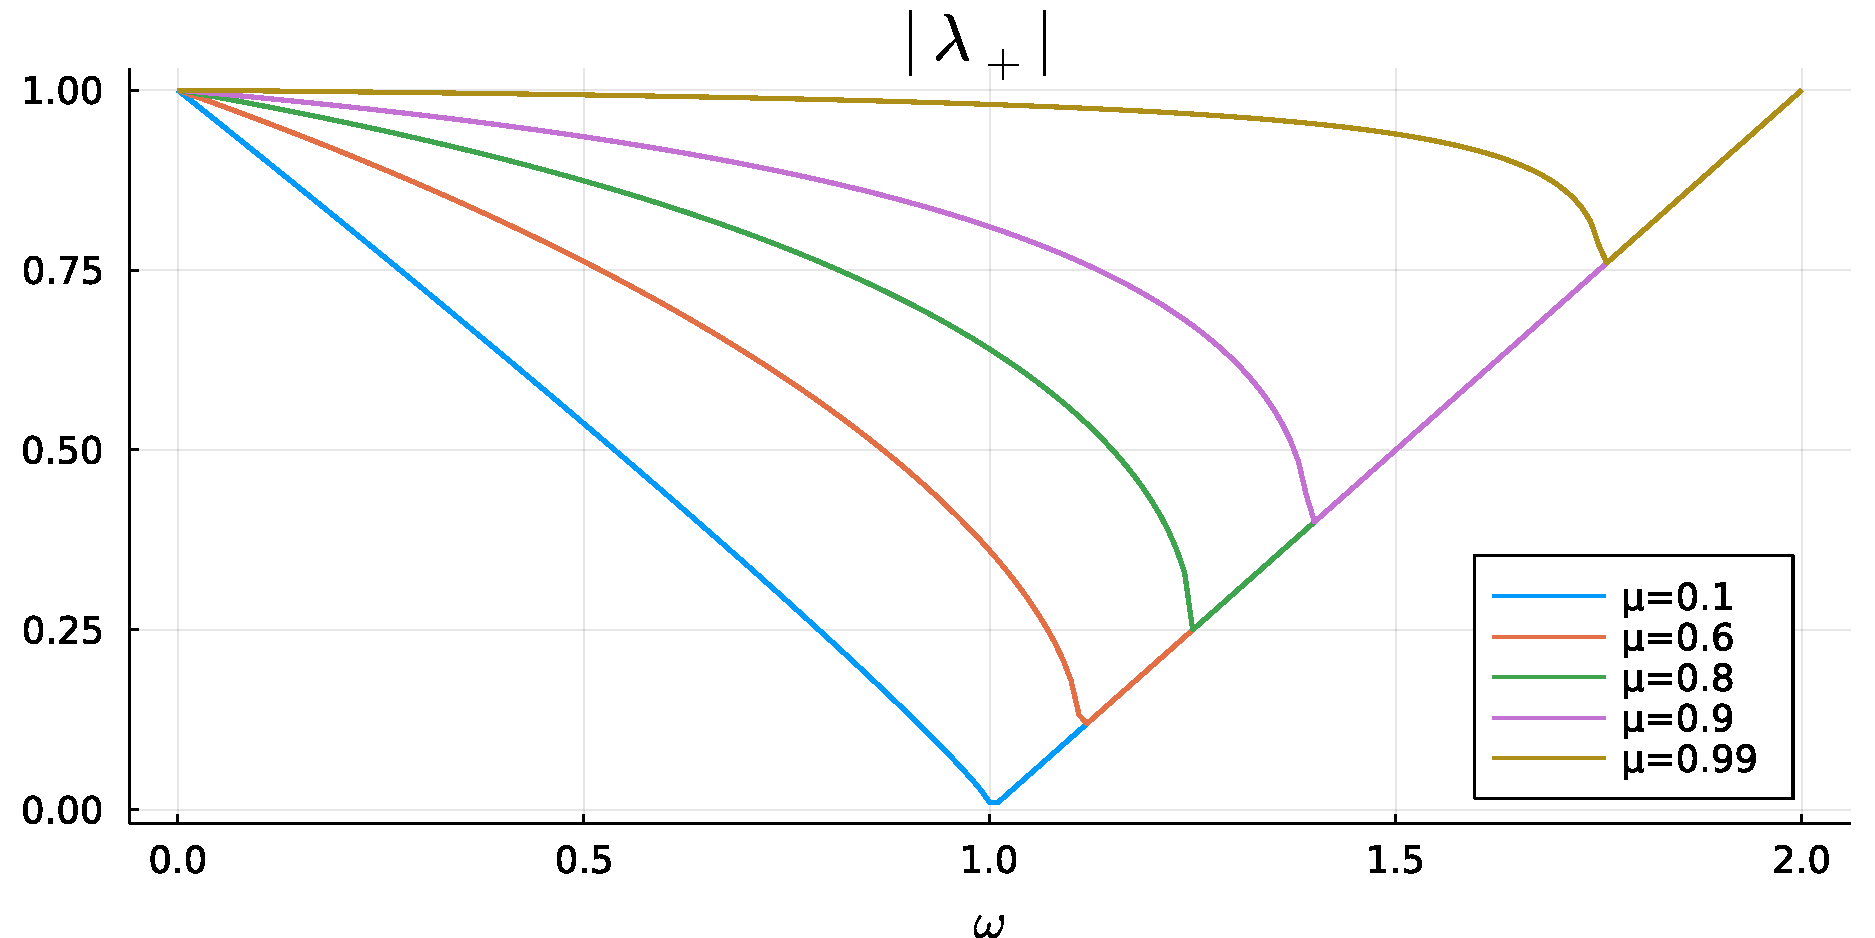
\includegraphics[width=0.8\linewidth]{figures/optimal_omega.pdf}
    \caption{Modulus of $\abs{\lambda_+}$ as a function of $\omega$,
    for different eigenvalues of $\mu$.}
    \label{fig:modulus_lambdas}
\end{figure}


\begin{exercise}
    [Midterm 2022]
    Let $\mat A \in \real^{n \times n}$ be a symmetric positive definite matrix and let~$\vect b \in \real^{n}$.
    The steepest descent algorithm for solving $\mat A \vect x = \vect b$ is given hereafter:

    \begin{center}
    \begin{algorithmic}
    \State Pick $\varepsilon > 0$ and initial $\vect x$%
    \State $\vect r \gets \mat A \vect x - \vect b$%
    \While{$\norm{\vect r} \geq \varepsilon \norm{\vect b}$}
        \State $\omega \gets \vect r^\t \vect r/\vect r^\t \mat A \vect r$
        \State $\vect x \gets \vect x - \omega \vect r$
        \State $\vect r \gets \mat A \vect x - \vect b$
    \EndWhile
    \end{algorithmic}
    \end{center}

    \noindent
    \begin{itemize}
        \item
            Why is this method called the \emph{steepest descent} algorithm?

        \item
            How many floating point operations does an iteration of this algorithm require?

        \item Are the following statements true of false? (2 marks)
        \begin{enumerate}
            \item
                There exists a unique solution~$\vect x_*$ to the linear system~\( \mat A \vect x = \vect b \).

            \item
                The iterates converge to $\vect x_*$ in at most $n$ iterations.

            \item
                We consider the following modification of the algorithm:
                \begin{center}
                \begin{algorithmic}
                \State Pick $\varepsilon > 0$, $\omega > 0$ and initial $\vect x$%
                \State $\vect r \gets \mat A \vect x - \vect b$%
                \While{$\norm{\vect r} \geq \varepsilon \norm{\vect b}$}
                    \State $\vect x \gets \vect x - \omega \vect r$
                    \State $\vect r \gets \mat A \vect x - \vect b$
                \EndWhile
                \end{algorithmic}
                \end{center}
                If $\omega$ is sufficiently small, then this algorithm converges.

            \item
                Here we no longer assume that $\mat A$ is positive definite.
                Instead, we consider that
                \[
                    \mat A =
                    \begin{pmatrix}
                        -1 & 0 \\ 0 & -2
                    \end{pmatrix}.
                \]
                In this case, the steepest descent algorithm is convergent for any initial $\vect x$.
        \end{enumerate}
    \end{itemize}
\end{exercise}

\begin{exercise}
    [Final exam Spring 2022]
    Assume that $\mat A \in \real^{n \times n}$ is a nonsingular matrix and that $\vect b \in \real^n$.
    We wish to solve the linear system~\eqref{eq:linear_system}
    using an iterative method where each iteration is of the form
    \begin{equation}
        \label{eq:iterative_scheme}
        \mat M \vect x_{k+1} = \mat N \vect x_k + \vect b.
    \end{equation}
    Here $\mat A = \mat M - \mat N$ is a splitting of~$\mat A$ such that $\mat M$ is nonsingular,
    and $\vect x_k \in \real^n$ denotes the $k$-th iterate of the numerical scheme.

    \begin{enumerate}
        \item
            Let $\vect e_k := \vect x_k - \vect x_*$,
            where $\vect x_*$ is the exact solution to~\eqref{eq:linear_system}.
            Prove that
            \[
                \vect e_{k+1} = \mat M^{-1} \mat N \vect e_k.
            \]

        \item
            Let $L = \norm{\mat M^{-1} \mat N}_{\infty}$.
            Prove that
            \begin{equation}
                \label{eq:inequality_interpolation}
                \forall k \in \nat, \qquad
                \norm{\vect e_k}_{\infty} \leq L^k \norm{\vect e_0}_{\infty}.
            \end{equation}

        \item
            Is the condition $\norm{\mat M^{-1} \mat N}_{\infty} < 1$ necessary
            for convergence when $\vect x_0 \neq \vect x_*$?

        \item
            Assume that $\mat A$ is strictly row diagonally dominant, in the sense that
            \[
                \forall i \in \{1, \dotsc, n\}, \qquad
                \lvert a_{ii} \rvert > \sum_{j=1, j\neq i}^{n} \lvert a_{ij} \rvert.
            \]
            Show that, in this case, the inequality $\norm{\mat M^{-1} \mat N}_{\infty} < 1$ holds for the Jacobi method,
            i.e.\ when $\mat M$ contains just the diagonal of~$\mat A$.
            You may take for granted the following expression for the~$\infty$-norm of a matrix $\mat X \in \real^{n \times n}$:
            \[
                \norm{\mat X}_{\infty} = \max_{1 \leq i \leq n} \sum_{j=1}^{n} \abs{x_{ij}}.
            \]

        \item
            Write down a few iterations of the Jacobi method when
            \[
                \mat A =
                \begin{pmatrix}
                    1 & 2 \\
                    0 & 1
                \end{pmatrix},
                \qquad
                \vect b
                \begin{pmatrix}
                    1 \\
                    1
                \end{pmatrix},
                \qquad
                \vect x_0 =
                \begin{pmatrix}
                    0 \\
                    0
                \end{pmatrix}.
            \]
            Is the method convergent?
    \end{enumerate}
\end{exercise}
